\documentclass{article}
% 编码设置
\usepackage[utf8]{inputenc}

% 页面布局和格式设置
\usepackage{geometry}
\geometry{a4paper, margin=1in} % 设置页面大小和边距

% 标题样式设置
\usepackage{titlesec}
\usepackage{xcolor} % 字体颜色
\usepackage{times} % 使用 Times New Roman 字体
\usepackage{fancyhdr} % 页眉和页脚设置
\usepackage{tabularx} % 用于更灵活的表格布局
\usepackage{array} % 更灵活地控制表格列宽
\usepackage{graphicx} % 插入图片
\usepackage{longtable} % 处理长表格
\usepackage{booktabs} % 增强表格的线条样式
\usepackage{amsmath} % 支持数学符号
\usepackage{caption} % 控制标题格式
\captionsetup[table]{skip=5pt} % 表格标题和表格内容的间距
\usepackage{enumitem} % 控制列表样式
\usepackage{amssymb} % 额外的数学符号
\usepackage{listings} % 格式化代码块
\usepackage{subcaption} % 支持子图表标题
\usepackage{float} % 强制位置选项
\usepackage{parskip} % 段落间距
\usepackage{pdflscape} % 支持横向页面
\usepackage{siunitx} % SI 单位支持
\usepackage{multirow} % 跨行单元格
\usepackage{mathpazo} % 数学字体
\usepackage{hyperref} % 超链接
\usepackage{cite} % 支持引用

% 页眉和页脚设置
\pagestyle{fancy}
\fancyhf{}
\fancyhead[L]{NUIST Experiment Report} % 左侧页眉显示报告标题
\fancyhead[R]{\thepage} % 右侧页眉显示页码

% 超链接设置
\hypersetup{
    colorlinks=true,
    linkcolor=blue,
    urlcolor=blue,
    pdftitle={NUIST Experiment Report}, % PDF 标题
    pdfauthor={Ziheng Wang} % PDF 作者信息
}

% 设置标题样式和分割线
\titleformat{\section}
  {\normalfont\Large}
  {\thesection.}{1em}{}
\titlespacing*{\section}{0pt}{1em}{0.5em}

% 自定义分割线命令
\newcommand{\sectionline}{%
  \noindent\textcolor{gray}{\rule{\textwidth}{0.5pt}}\par\vspace{1em}
}

% 代码块样式设置
\lstset{
    basicstyle=\ttfamily\footnotesize,
    breaklines=true,
    frame=single,
    numbers=left,
    numberstyle=\tiny,
    xleftmargin=2em,
    framexleftmargin=1.5em,
    tabsize=4,
    showstringspaces=false
}

\begin{document}

% 封面标题
\begin{center}
    {\LARGE \textbf{NUIST Experiment Report}}
\end{center}
\sectionline % 标题下的分割线

\vspace{1em}

% 信息表格
\large % 使表格字体变大
\begin{tabularx}{\textwidth}{>{\raggedright\arraybackslash}X l}
    \textbf{Course name:} & \\[1em]
    \textbf{Experiment name:} & \\[1em]
    \textbf{Date:} & \hspace{4em} \textbf{Tutor:} \\[1em]
    \textbf{College:} & \hspace{4em} \textbf{Class:} \\[1em]
    \textbf{Name:} & \\[1em]
    \textbf{Student ID:} & \\
\end{tabularx}
\normalsize % 恢复正常字体大小

\vspace{1em}

% 1. 实验分工部分
\section{Experimental Division of Labor}
\sectionline % 分割线
% 在这里列出实验分工
\begin{itemize}[leftmargin=*, labelsep=1em]
    \item \textbf{Name 1}: Contribution 1
    \item \textbf{Name 2}: Contribution 2
\end{itemize}

% 2. 实验内容部分
\section{Experimental Content}
\sectionline % 分割线
% 在这里描述实验内容,包括方法、公式、程序结构等
\textbf{Method Introduction:} Describe the experimental method here.

\textbf{Formula Introduction:}
\begin{equation}
    E = mc^2
\end{equation}

\textbf{Program Structure:} Outline the program structure here.

\textbf{Flow Chart:}
\begin{figure}[H]
    \centering
    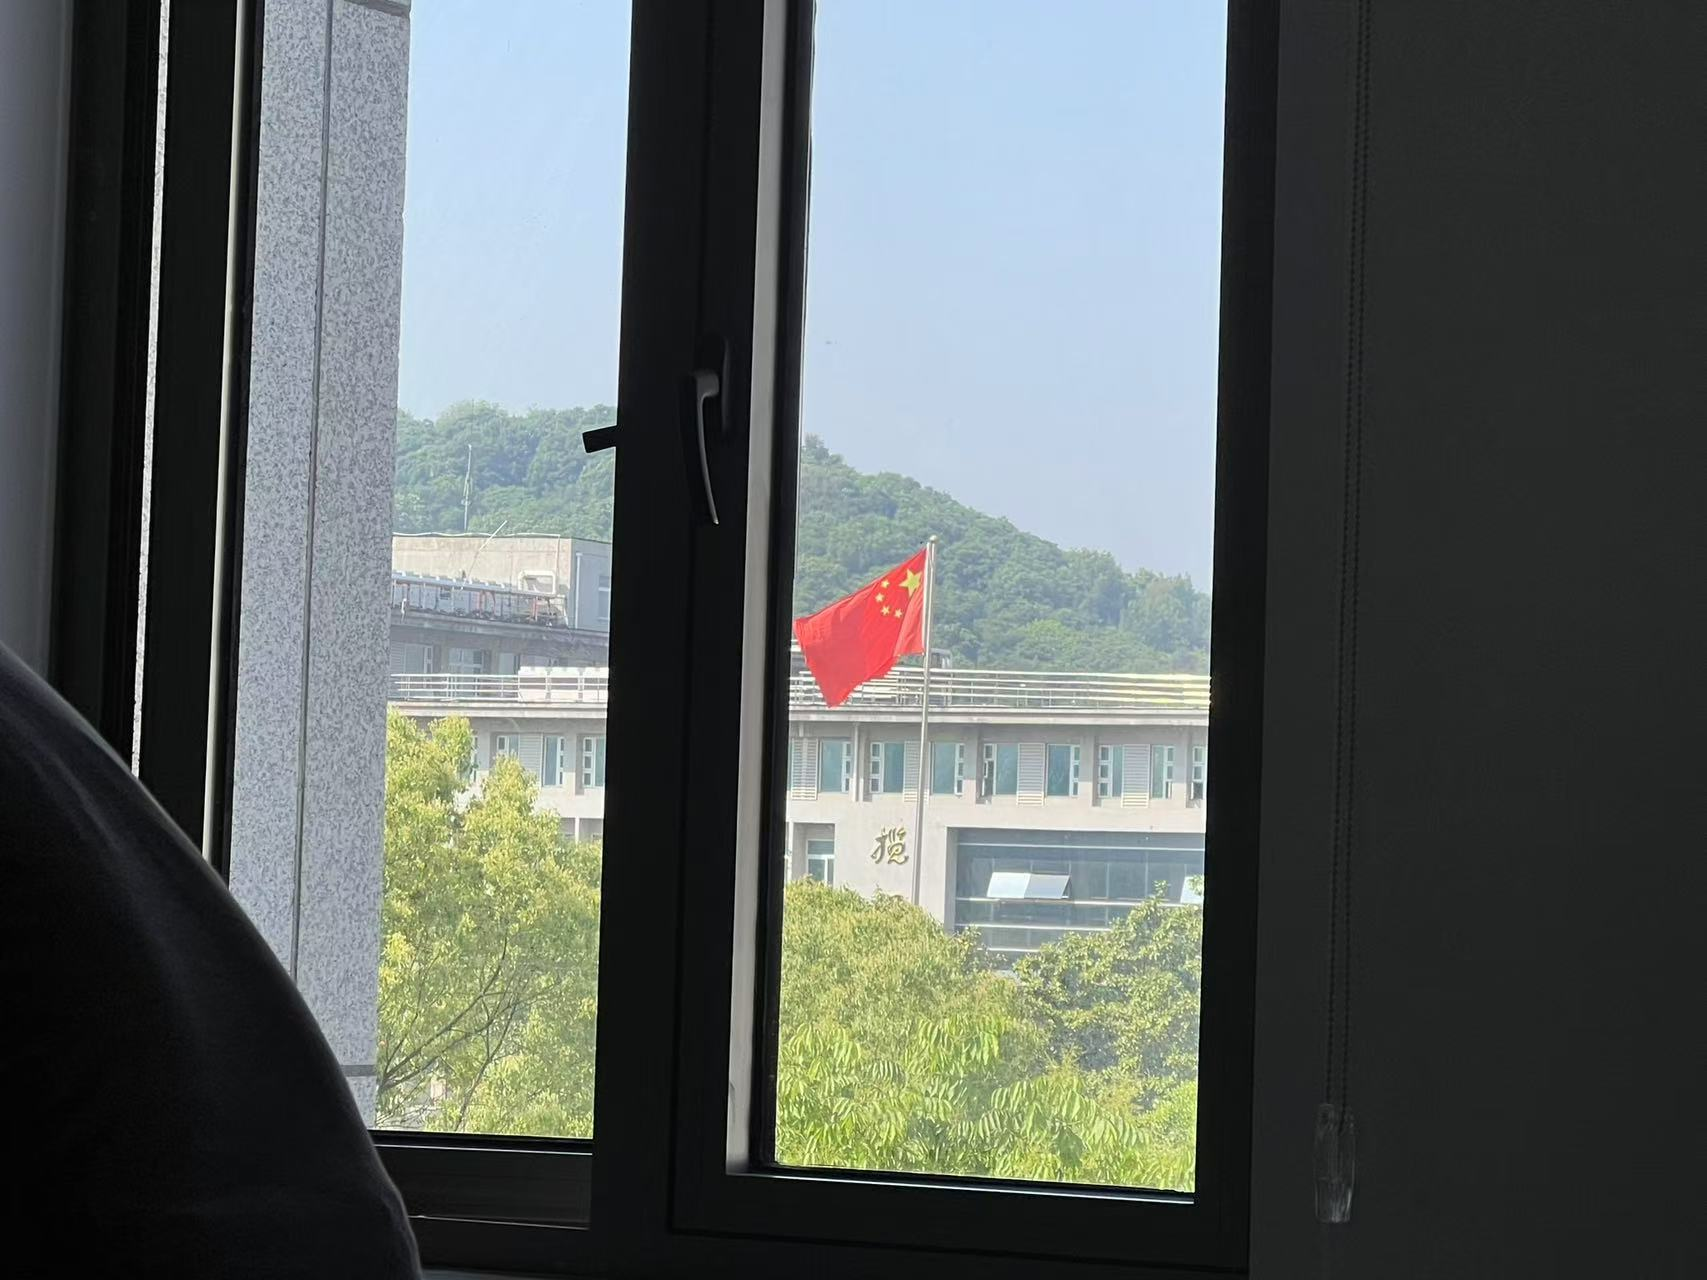
\includegraphics[width=0.7\textwidth]{flowchart.png}
    \caption{Flow Chart of Experimental Procedure}
\end{figure}

% 3. 实验结果部分
\section{Experimental Result}
\sectionline % 分割线
% 在此处包含实验结果的截图和分析
\begin{figure}[H]
    \centering
    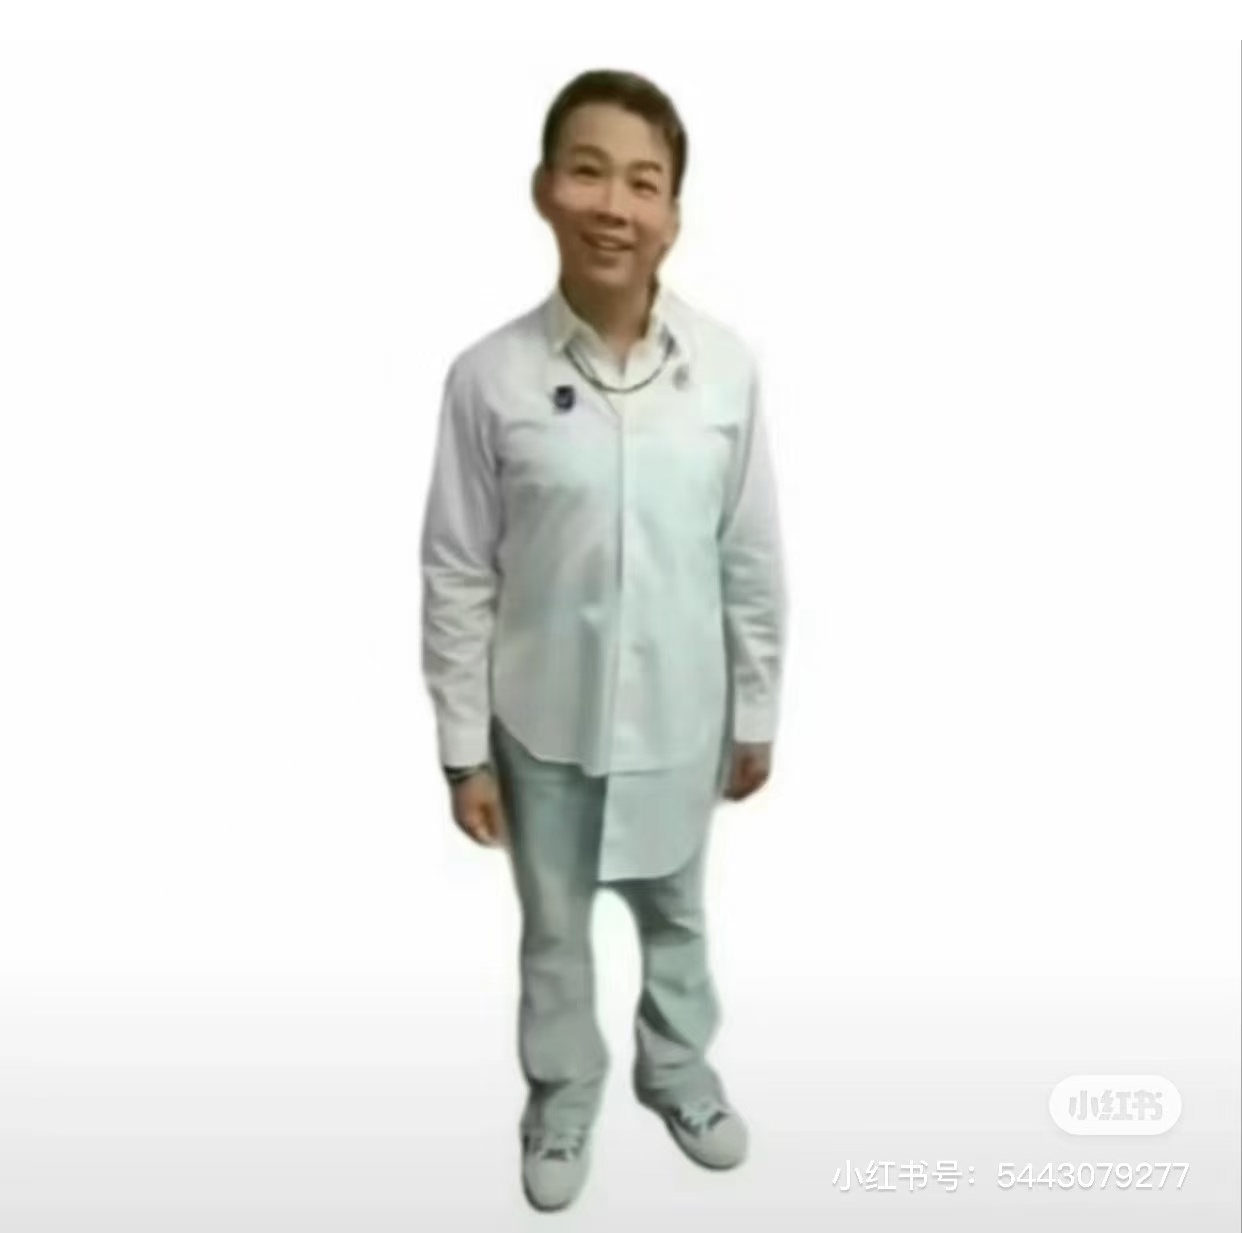
\includegraphics[width=0.8\textwidth]{result.png}
    \caption{Example of Experimental Result}
\end{figure}

\textbf{Analysis:} Provide an analysis of the experimental results.

% 4. 程序代码部分
\section{Program Code}
\sectionline % 分割线
% 列出实验程序的代码,保持代码缩进
\begin{lstlisting}[language=Python, caption={Sample Code}]
# Crested Porcupine Optimizer implementation
def optimizer():
    # Code logic here
    pass
\end{lstlisting}

% 5. 结论部分
\section{Conclusions}
\sectionline % 分割线

% 提示:请在结论部分引用本模板的 GitHub 项目地址。
% 引用方法:
% 1. 确保当前项目文件夹中有 references.bib 文件。
% 2. 在 references.bib 文件中加入以下 BibTeX 条目。
% 
% @misc{wang2024nuist,
%   author       = {Ziheng Wang},
%   title        = {NUIST Experiment Report LaTeX Template},
%   year         = {2024},
%   url          = {\url{https://github.com/Nickory/Nuist-expriment-report-latex}},
%   note         = {Available at GitHub: \url{https://github.com/Nickory/Nuist-expriment-report-latex}},
% }
%
% 3. 使用 \cite{wang2024nuist} 在结论部分进行引用。
% 示例:在实验过程中使用了 NUIST 实验报告模板,详细信息参见 \cite{wang2024nuist}。

Discuss any issues encountered, solutions, insights, and suggestions related to the experiment. 

\cite{wang2024nuist} % 记得在 references.bib 文件中添加相应的条目以正确引用

% 6. 引用部分
\section{References}
\sectionline % 分割线

\bibliographystyle{plain}
\bibliography{ref} % 在当前文件夹中添加一个 refs.bib 文件并填入文献信息

% 制作者信息
% Author: Ziheng Wang
% Contact: zhwang@nuist.edu.cn
% GitHub: https://github.com/Nickory/Nuist-expriment-report-latex

\end{document}
